\batchmode
\makeatletter
\def\input@path{{C:/Users/wrbrooks/git/beauty_contest/writeup//}}
\makeatother
\documentclass{article}\usepackage[]{graphicx}\usepackage[]{color}
%% maxwidth is the original width if it is less than linewidth
%% otherwise use linewidth (to make sure the graphics do not exceed the margin)
\makeatletter
\def\maxwidth{ %
  \ifdim\Gin@nat@width>\linewidth
    \linewidth
  \else
    \Gin@nat@width
  \fi
}
\makeatother

\definecolor{fgcolor}{rgb}{0.345, 0.345, 0.345}
\newcommand{\hlnum}[1]{\textcolor[rgb]{0.686,0.059,0.569}{#1}}%
\newcommand{\hlstr}[1]{\textcolor[rgb]{0.192,0.494,0.8}{#1}}%
\newcommand{\hlcom}[1]{\textcolor[rgb]{0.678,0.584,0.686}{\textit{#1}}}%
\newcommand{\hlopt}[1]{\textcolor[rgb]{0,0,0}{#1}}%
\newcommand{\hlstd}[1]{\textcolor[rgb]{0.345,0.345,0.345}{#1}}%
\newcommand{\hlkwa}[1]{\textcolor[rgb]{0.161,0.373,0.58}{\textbf{#1}}}%
\newcommand{\hlkwb}[1]{\textcolor[rgb]{0.69,0.353,0.396}{#1}}%
\newcommand{\hlkwc}[1]{\textcolor[rgb]{0.333,0.667,0.333}{#1}}%
\newcommand{\hlkwd}[1]{\textcolor[rgb]{0.737,0.353,0.396}{\textbf{#1}}}%

\usepackage{framed}
\makeatletter
\newenvironment{kframe}{%
 \def\at@end@of@kframe{}%
 \ifinner\ifhmode%
  \def\at@end@of@kframe{\end{minipage}}%
  \begin{minipage}{\columnwidth}%
 \fi\fi%
 \def\FrameCommand##1{\hskip\@totalleftmargin \hskip-\fboxsep
 \colorbox{shadecolor}{##1}\hskip-\fboxsep
     % There is no \\@totalrightmargin, so:
     \hskip-\linewidth \hskip-\@totalleftmargin \hskip\columnwidth}%
 \MakeFramed {\advance\hsize-\width
   \@totalleftmargin\z@ \linewidth\hsize
   \@setminipage}}%
 {\par\unskip\endMakeFramed%
 \at@end@of@kframe}
\makeatother

\definecolor{shadecolor}{rgb}{.97, .97, .97}
\definecolor{messagecolor}{rgb}{0, 0, 0}
\definecolor{warningcolor}{rgb}{1, 0, 1}
\definecolor{errorcolor}{rgb}{1, 0, 0}
\newenvironment{knitrout}{}{} % an empty environment to be redefined in TeX

\usepackage{alltt}
\usepackage[T1]{fontenc}
\usepackage[latin9]{inputenc}
\usepackage{geometry}
\geometry{verbose,tmargin=2cm,bmargin=2cm,lmargin=2cm}
\setlength{\parskip}{\bigskipamount}
\setlength{\parindent}{0pt}
\synctex=-1
\usepackage{bm}
\usepackage{amsthm}
\usepackage{amsmath}
\usepackage{setspace}
\usepackage[authoryear]{natbib}
\doublespacing

\makeatletter
%%%%%%%%%%%%%%%%%%%%%%%%%%%%%% Textclass specific LaTeX commands.
\numberwithin{equation}{section}
\numberwithin{figure}{section}

%%%%%%%%%%%%%%%%%%%%%%%%%%%%%% User specified LaTeX commands.
\renewcommand\[{\begin{equation}}
\renewcommand\]{\end{equation}}
\usepackage{subfig}
\usepackage{rotating}

\makeatother

\usepackage[english]{babel}
\IfFileExists{upquote.sty}{\usepackage{upquote}}{}
\begin{document}

\title{Beauty Contest}


\author{Wesley Brooks, Steve Corsi, Rebecca Carvin}
\maketitle
\begin{abstract}
Pithy, concise and informative. May bring the reader to tears due
to the beauty of it.
\end{abstract}

\section{Introduction}


\section{Methods}

The availability of large data sets for building regression models
to predict the bacterial counts in beach water is both an opportunity
and a challenge. 


\subsection{Data Sources}

\emph{Possibly move this to the end of the section}

Which sites

Where are they

What specific sources sources of data (plug EnDDAT)

Will include a map and tables


\subsection{Definitions}

At any site, denote the predictor variables by $X$, which is an $n\times p$
matrix where $n$ is the number of observations and $p$ is the number
of predictors. The vector of $n$ observations of bacterial concentration
is denoted $y$. The mathematical model relating $y$ to $X$ is the
function $\mu(X,$y).


\subsection{Goals}

With input from the US Environmental Protection Agency, the state
of Wisconsin has established regulatory standards for beach water
quality, which states that a warning is to be posted when the concentration
of E. coli exceeds 235 CFU / 100 mL.  The goal of modeling the bacterial
concentration is to predict in advance when the concentration will
exceed the limit. For the discussion to come, denote the regulatory
standard by $\delta$. Each model has two essential components: the
mathematical model itself, $\mu(X,y)$, and a decision threshold,
$\hat{{\delta}}$, that is used to interpret the model's predictions.

There is no reason that $\delta$ and $\hat{{\delta}}$ must be equal.
Rather, each $\hat{{\delta}}$ should be chosen so that the number
of false positives and false negatives are balanced to the satisfaction
of the beach manager. Using cross validation allows us to set $\hat{{\delta}}$
to expect that the performance over future data will resemble what
was observed over the testing data.


\subsection{Listing of specific statistical techniques}

Fourteen different regression modeling techniques were considered.
Each technique uses one of five modeling algorithms: GBM, the adaptive
lasso, the genetic algorithm, PLS, or sparse PLS. Each technique is
applied to either continuous or binary regression and to either variable
selection and model estimation, or variable selection only.


\subsubsection*{Continuous vs. binary regression}

The goal of predicting exceednaces of the water quality standard is
approached in two ways: one is to predict the bacterial concentration
and then compare the prediction to a threshold, which is referred
to as continuous modeling. The other is referred to as binary modeling,
in which we predict the state of the binary indicator $z_{i}$:

\[
z_{i}=I(y_{i}>\delta)
\]


The indicator is coded as zero when the concetration is below the
regulatory standard and one when the concentration exceeds the standard.
All of the binary modeling techniques herein use logistic regression,
which uses the logistic link function $g$ to translate $p_{i}=E(z_{i})$
- the probability that the $i$th observation is an exceedance - into
an unbounded quantity.

\[
g(p_{i})=\log\frac{p_{i}}{1-p_{i}}
\]



\paragraph*{Weighting of observations in binary regression}

A weighting scheme was implemented for some of the binary regression
techniques. In the weighting scheme, observations were given weights
$w_{i}$ where:

\begin{align*}
w_{i}= & (y_{i}-\delta)/\hat{{sd}}(y)\\
\hat{{sd}}(y)= & \sqrt{\sum_{i=1}^{n}(y_{i}-\bar{{y}})^{2}/n}\\
\bar{{y}}= & \sum_{i=1}^{n}y_{i}/n
\end{align*}


That is, the weights are equal to the number of standard deviations
that the observed concentration lies from the regulatory threshold
$\delta$. Any technique that was implemented with this weighting
scheme was separately implemented without any weighting of the observations.
The techniques are thus labeled weighted and unweighted, respectively.


\subsubsection*{Modeling or selection only}

The regression techniques adaptive lasso and sparse PLS include a
variable selection step. , Some methods are labeled ``select'',
which means that they are used for variable selection only. In these
cases, once the predictor variables are selected, the regression model
using those predictors is estimated using ordinary least squares for
the continuous regression techniques, or ordinary logistic regression
for the binary regression techniques.


\subsubsection{GBM}

GBM refers to the gradient boosting machine (GBM) of \citet{Friedman-2001}.
A GBM model is a so-called random forest model - a collection of many
regression trees. Prediction is done by averaging the outputs of the
trees. Two GBM-based techniques are explored - we refer to them as
GBM and GBMCV. The difference is in how the optimal number of trees
is determined - GBMCV selects the number of trees in a model using
leave-one-out CV, while GBM uses the so-called out-of-bag (OOB) error
estimate. The CV method is much slower (it has to construct as many
random forests as there are observations, while the OOB method only
requires computing a single random forest) but GBMCV should more accurately
estimate the prediction error. All the GBM and GBMCV models share
the following settings:

Number of trees: 10000

Shrinkage parameter: 0.0005

Minimum observations per node: 5

Depth of each tree: 5

Bagging fraction: 0.5


\subsubsection{Adaptive Lasso}

The adaptive lasso \citep{Zou-2006} is a regression method that simultaneously
selects relevant predictors and estimates their coefficients by adding
a penalty to the sum of the squared residuals. For continuous modeling
techniques the adaptive lasso selects the predictors for linear regression,
estimating $\hat{{\bm{\beta}}}$ minimize the criterion $\sum_{i=1}^{n}(y_{i}-X_{i}\beta)^{2}+\lambda\sum_{j=1}^{p}\frac{{|\beta_{j}|}}{\tilde{{|\beta_{j}|^{\gamma}}}}$,
where $\lambda$ is a tuning parameter and $\tilde{{\bm{\beta}}}$
is a consistent estimate of the regression coefficients.

For binary modeling, the adaptive lasso maximizes the penalized log-likelihood
$\sum_{i=1}^{n}\left[-\left(1-y_{i}\right)X_{i}\beta-\log\left\{ 1+\exp\left(-X_{i}\beta\right)\right\} \right]+\lambda\sum_{j=1}^{p}\frac{{|\beta_{j}|}}{\tilde{{|\beta_{j}|^{\gamma}}}}$,
where, as was the case for continuous response, $\tilde{\bm{\beta}}$
is a consistent estimate of the regression coefficients, which is
calculated by ordinary logistic regression.

In this work, $\gamma=1$ , $\tilde{{\bm{\beta}}}$ are estimated
individually by a univariate linear or logistic regression (it is
necessary to estimate the coefficients individually because there
are usually more covariates than observations), and the adaptive lasso
tuning parameter $\lambda$ is selected to minimize the AICc \citep{Hurvich-Simonoff-Tsai-1998}.

Five of the modeling techniques were based on the adaptive lasso -
one for continuous response (AL), and four for binary response (AL-logistic-weighted,
AL-logistic-unweighted, AL-logistic-weighted-select, AL-logistic-unweighted-select).
The four binary response techniques are the combination of weighted
versus unweighted, and selection-only versus selection-and-estimation.


\subsubsection{Genetic algorithm}

The genetic algorithm \citep{Fogel-1998} is a variable-selection
method that works by analogy to natural selection, where so-called
chromosomes represent regression models. A variable is included in
the model if the corresponding element of the chromosome is one, but
not otherwise. Chromosomes are produced in successive generations,
where the first generation is produced randomly and subsequent generations
are produced by combining chromosomes from the current generation,
with additional random drift. The chance that a chromosome in the
current generation will produce offspring in the next generation is
an increasing function of its fitness. The fitness of each chromosome
is calculated by the corrected Akaike Information Criterion (AICc)
\citet{Akaike-1973,Hurvich-Tsai-1989}.

The implementations in this study used 100 generations, with each
generation consisting of 200 chromosomes. The genetic algorithm method
(GA) is the default for linear regression modeling in Virtual Beach
\citep{Cyterski-Brooks-Galvin-Wolfe-Carvin-Roddick-Fienen-Corsi-2013}.
This study also investigates two genetic algorithm methods for logistic
regression: one weighted (GA-logistic-weighted) and one unweighted
(GA-logistic-unweighted).


\subsubsection{PLS}

Partial least squares (PLS) regression is a tool for building regression
models with many covariates \citep{Wold-Sjostrum-Eriksson-2001}.
PLS works by decomposing the covariates into mutually orthogonal components,
with the components then used as the variables in a regression model.
This is similar to principal components regression (PCR), but the
way PLS components are chosen ensures that they are aligned with the
model output. On the other hand, PCR is sometimes criticised for decomposing
the covariates into components that are unrelated to the model's output.

To use PLS, one must decide how many components to use in the model.
This study follows the method described in \citet{Brooks-Fienen-Corsi-2013},
using the PRESS statistic to select the number of components.


\subsubsection{SPLS}

Sparse PLS (SPLS) is introduced in \citet{Chun-Keles-2007}. The SPLS
method combines the orthogonal decompositions of PLS with the sparsity
of lasso-type variable selection. To do so, SPLS uses two tuning parameters:
one that controls the number of orthogonal components and one that
controls the lasso-type penalty. The optimal parameters are those
that minimize the mean squared prediction error (MSEP) over a two-dimensional
grid search. The MSEP is estimated by 10-fold cross-validation. SPLS
was used for both selection-and-estimation (SPLS) and selection-only
(SPLS-select).


\subsection{Implementation for beach regression}

The response variable for our continuous regression models is the
natural logarithm of the E. coli concentration. For the binary regression
models, the response variable is an indicator of whether the concentration
exceeds the regulatory threshold $\delta=235$ CFU/mL.Some pre-processing
of the data was done. During pre-processing, some transformations
were applied to the data. The beach water turbidity and the discharge
of tributaries near each beach were log-transformed. Rainfall variables
were all square-root transformed.

Include a table with pre/post processing discussion

\begin{knitrout}
\definecolor{shadecolor}{rgb}{0.969, 0.969, 0.969}\color{fgcolor}\begin{kframe}


{\ttfamily\noindent\bfseries\color{errorcolor}{\#\# Error: unable to find an inherited method for function '[' for signature '"{}dgCMatrix"{}'}}

{\ttfamily\noindent\bfseries\color{errorcolor}{\#\# Error: object 'press.meanranks' not found}}\end{kframe}
\end{knitrout}


\section{Results}


\subsection{Results tables}

Results of the cross-validation procedures were compiled into tables

\begin{table}
	\centering
	\begin{tabular}{ccccc}
<<results-table, echo=FALSE, warning=FALSE, message=FALSE, results='asis'>>
	#Generate an example results table
	
	#First, get the reults from hika, bot LOO and LOYO:
	r = results[['hika']][['gbm']][['res']]
	ra = results_annual[['hika']][['gbm']][['res']]

	#Find the original ordering of the data:
	r %>% rownames %>% as.integer %>% order -> indx
	ra %>% rownames %>% as.integer %>% order -> indx_annual

	#Produce a results table:
	rtable = cbind(r[indx,c(2,1,3)], ra[indx_annual,c(1,3)])[1:4,]
	colnames(rtable) = c("Actual",
		"\\begin{tabular}{c}LOO\\\\prediction\\end{tabular}",
		"\\begin{tabular}{c}LOO\\\\threshold\\end{tabular}",
		"\\begin{tabular}{c}LOYO\\\\prediction\\end{tabular}",
		"\\begin{tabular}{c}LOYO\\\\threshold\\end{tabular}")
	
	#Add ellipses for the last row:
	rtable = rtable %>% round(2) %>%
		rbind(rep("\\vdots", 5))

	#Display only a summary:
	rtable %>% xtable %>% print(only.content=TRUE)
@
	\end{tabular}
\end{table}


\subsection{Cross Validation}

Our assessment of the modeling techniques is based on their performance
in predicting exceedances of the regulatory standard. Two types of
cross validation was used to measure the performance in prediction:
leave-one-out (LOO) and leave-one-year-out (LOYO). In LOO CV, one
observation is held out for validation while the rest of the data
is used to train a model. The model is used to predict the concentration
of that held out observation, and the process is repeated for each
observation. Each cycle of LOYO CV holds out an entire year's worth
of data for validation instead of a single observation. It is intended
to approximate the performance of the modeling technique under a typical
use case: a new model is estimated before the start of each annual
beach season and then used for predicting exceedances during the season.
The LOYO models in this study were estimated using all the available
data except for the held out year, even that from future years. So
for instance the 2012 models were estimated using the 2010-2011 and
2013 data.

Some methods also used cross-validation internally to select tuning
parameters. In those cases the internal CV was done using only the
model data, and never looking at the held-out observation(s). This
process is separate from - and does not affect - the CV to assess
predictive performance.


\subsection{Comparing methods, and quantifying uncertainty in the ranks}

Our goal is to compare the different modeling techniques. We make
comparisons on the basis of rank because the modeling metrics may
not be comparable between sites (because, for instance, different
sites have different numbers of observations). If it is possible to
compute a metric of model performance, then it is possible to rank
the techniques based on that metric. Our approach is to rank the techniques
at each site (higher is better), and then average the ranks of each
method.

In order tocompare techniques, we must quantify the uncertainty in
the rankings, which we do via the bootstrap. Since the AUROC and PRESS
rankings are functions of the result tables, the bootstrap procedure
is carried out by resampling the rows of each results table, and the
AUROC and ROC rankings were recalculated for each bootstrap sample.
We used $1001$ bootstrap samples of each results table in the analysis
that follows.


\subsection{AUROC}

The receiver operating characteristic (ROC) curve is a graphical display
of how well predictions are sorted. Each point on the curve represents
the model's performance for a specific choice of the threshold $\hat{\delta}$
in terms of specificity and sensitivity. A model with well-sorted
predictions is one where the predicted bacterial contentration (or
the predicted probability of exeedance in the case of a binary regression
model) is consistently greater when the true concentration exceeds
the regulatory standard than when it does not. In such a case, the
model may have both good sensitivity and good specificity over a wide
range of thresholds $\hat{\delta}$.

The area under the ROC curve (AUROC) summarizes the model's performance
over the range of possible thresholds. A model which perfectly separates
exceedances from non-exceedances in prediction has an AUROC of one,
while a model that predicts exceedances no better than a coin flip
has an AUROC of 0.5.

The methods are ranked at each site by AUROC and a mean rank (across
sites) is computed for each method. The mean LOO and LOYO ranks are
plotted in Figure \ref{fig:auroc-boxplot}. The top three techniques
were GBM, GBM-CV and adaptive lasso. In order to facilitate a pairwise
comparison between modeling methods, Tables \ref{table:auroc.pairs.annual}
(for the leave-one-year-out analysis) and \ref{table:auroc.pairs}
(for the leave-one-out analysis) show the frequency that the mean
AUROC rank of GBM, GBM-CV, or the adaptive lasso exceeded each of
the other modeling methods.

\begin{knitrout}
\definecolor{shadecolor}{rgb}{0.969, 0.969, 0.969}\color{fgcolor}\begin{kframe}


{\ttfamily\noindent\bfseries\color{errorcolor}{\#\# Error: error in evaluating the argument 'x' in selecting a method for function 'print': Error: object 'roc.barchart' not found}}\end{kframe}\begin{figure}[]

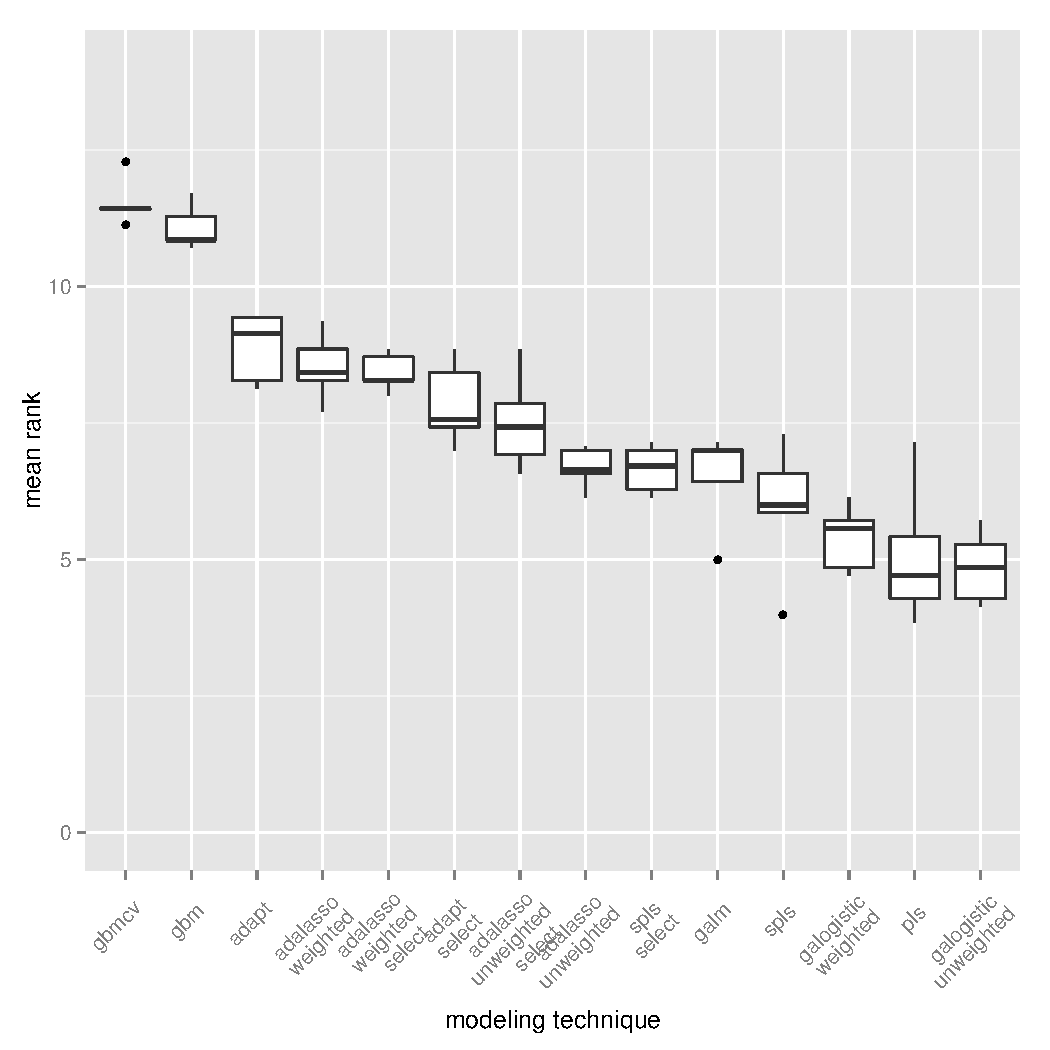
\includegraphics[width=0.49\linewidth]{figure/auroc-boxplot} \caption[Mean ranking of the methods by area under the ROC curce (AUROC) across all sites (higher is better)]{Mean ranking of the methods by area under the ROC curce (AUROC) across all sites (higher is better). The error bars are 90\% confidence intervals computed by the bootstrap. At left are the AUROC rankings from the leave-one-year-out cross validation, at right are the AUROC rankings from the leave-one-out cross validation.\label{fig:auroc-boxplot}}
\end{figure}


\end{knitrout}

% latex table generated in R 3.0.2 by xtable 1.7-1 package
% Mon Jul 28 14:51:39 2014
\begin{table}[ht]
\centering
\begin{tabular}{rrrrrrrrrrrrrr}
  \hline
 & \begin{sideways} \begin{tabular}{l}gbmcv\end{tabular} \end{sideways} & \begin{sideways} \begin{tabular}{l}adapt\end{tabular} \end{sideways} & \begin{sideways} \begin{tabular}{l}spls\end{tabular} \end{sideways} & \begin{sideways} \begin{tabular}{l}adalasso \\ weighted\end{tabular} \end{sideways} & \begin{sideways} \begin{tabular}{l}spls \\ select\end{tabular} \end{sideways} & \begin{sideways} \begin{tabular}{l}adalasso \\ unweighted\end{tabular} \end{sideways} & \begin{sideways} \begin{tabular}{l}pls\end{tabular} \end{sideways} & \begin{sideways} \begin{tabular}{l}adapt \\ select\end{tabular} \end{sideways} & \begin{sideways} \begin{tabular}{l}adalasso \\ unweighted \\ select\end{tabular} \end{sideways} & \begin{sideways} \begin{tabular}{l}adalasso \\ weighted \\ select\end{tabular} \end{sideways} & \begin{sideways} \begin{tabular}{l}galogistic \\ weighted\end{tabular} \end{sideways} & \begin{sideways} \begin{tabular}{l}galogistic \\ unweighted\end{tabular} \end{sideways} & \begin{sideways} \begin{tabular}{l}galm\end{tabular} \end{sideways} \\ 
  \hline
gbm & 1.00 & 1.00 & 1.00 & 1.00 & 1.00 & 1.00 & 1.00 & 1.00 & 1.00 & 1.00 & 1.00 & 1.00 & 1.00 \\ 
  gbmcv &  & 0.67 & 1.00 & 1.00 & 1.00 & 1.00 & 1.00 & 0.67 & 1.00 & 1.00 & 1.00 & 1.00 & 1.00 \\ 
  adapt &  &  & 0.67 & 0.67 & 0.67 & 0.67 & 1.00 & 1.00 & 1.00 & 1.00 & 1.00 & 1.00 & 1.00 \\ 
   \hline
\end{tabular}
\caption{Under leave-one-year-out cross validation, how often the mean AUROC rank of GBM, GBMCV, or the adaptive lasso (in the rows) exceeded that of the other methods (in the columns).} 
\label{table:auroc.pairs.annual}
\end{table}
\begin{kframe}

{\ttfamily\noindent\bfseries\color{errorcolor}{\#\# Error: object 'auroc.pairs' not found}}\end{kframe}


\subsection{PRESS}

While AUROC is concerned with how well the model's predictions separate
exceedances from non-exceedances, the predictive error sum of squares
(PRESS) measures how well a model's predictions match the observed
bacterial concentration. The PRESS can only be computed for continuous
regression methods. Let the model's predictions be denoted $\tilde{y}_{i}$
and letting the actual observed bacterial concentrations be denoted
$y_{i}$ for $i=1,\dots,n$ where $n$ is the total number of predictions.
Then PRESS computed as follows:

\[
\text{PRESS}=\sum_{i=1}^{n}\left(\tilde{y}_{i}-y_{i}\right)^{2}.
\]


The PRESS statistic is of interest because a good model should accurately
predict the bacterial concentration, and a model that more accurately
predicts the concentration may be easier to trust. However, the AUROC
is a more important as a metric of model performance than the PRESS
because it directly measures the ability of a model to separate exceedances
from non-exceedances. That said, we expect the two statistics to usually
agree on which modeling methods are the best.

The rankings of the methods by PRESS are plotted in Figure \ref{fig:press-boxplot}.
The top three techniques under both LOO and LOYO analysis were GBM,
GBM-CV and the adaptive lasso. In order to facilitate a pairwise comparison
between modeling methods, Tables \ref{table:auroc.pairs.annual} (for
the leave-one-year-out analysis) and \ref{table:auroc.pairs} (for
the leave-one-out analysis) show the frequency that the mean AUROC
rank of GBM, GBM-CV, or the adaptive lasso exceeded each of the other
modeling methods.

\begin{knitrout}
\definecolor{shadecolor}{rgb}{0.969, 0.969, 0.969}\color{fgcolor}\begin{kframe}


{\ttfamily\noindent\bfseries\color{errorcolor}{\#\# Error: error in evaluating the argument 'x' in selecting a method for function 'print': Error: object 'press.barchart' not found}}\end{kframe}\begin{figure}[]

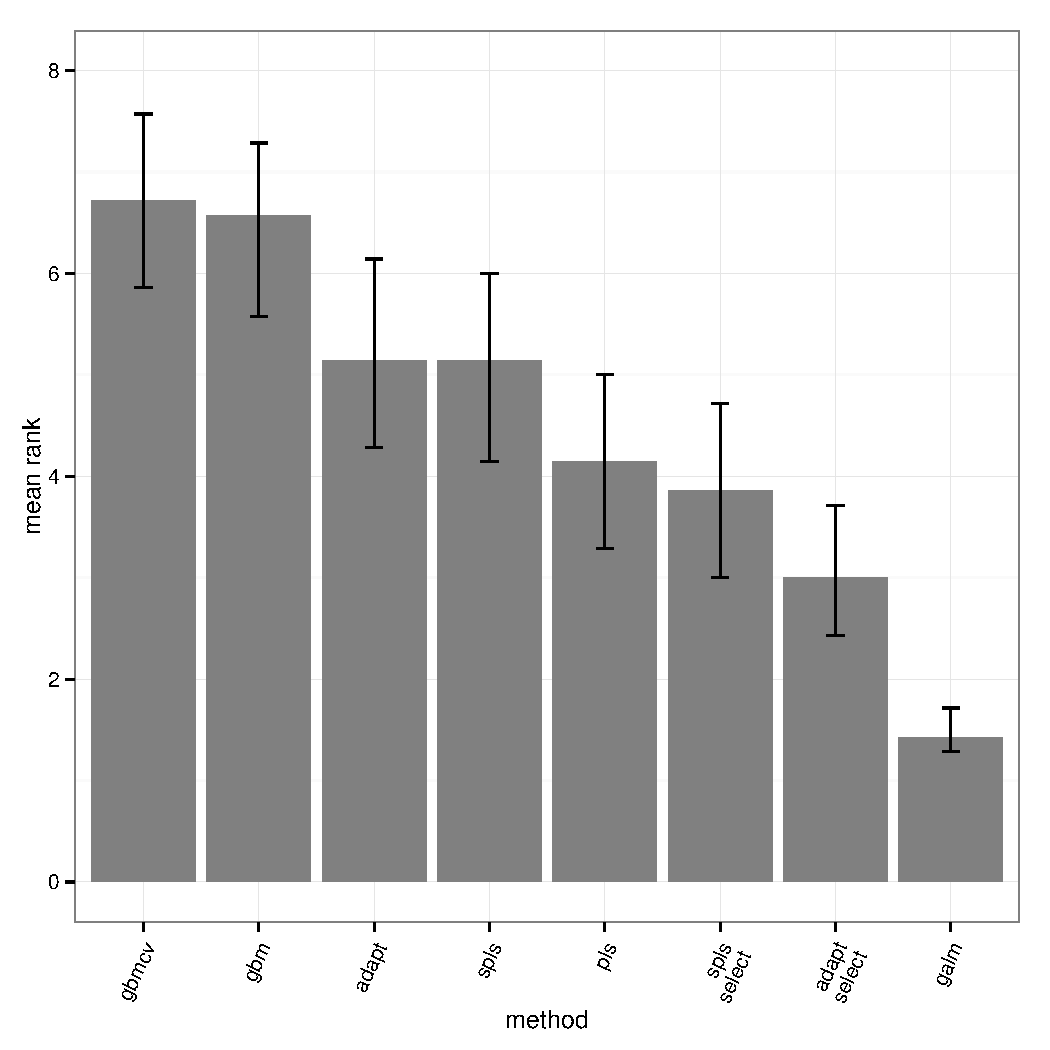
\includegraphics[width=0.49\linewidth]{figure/press-boxplot} \caption[Mean ranking of the methods by predictive error sum of squares (PRESS) across all sites (higher is better)]{Mean ranking of the methods by predictive error sum of squares (PRESS) across all sites (higher is better). The error bars are 90\% confidence intervals computed by the bootstrap. At left are the PRESS rankings from the leave-one-year-out cross validation, at right are the PRESS rankings from the leave-one-out cross validation.\label{fig:press-boxplot}}
\end{figure}


\end{knitrout}

% latex table generated in R 3.0.2 by xtable 1.7-1 package
% Mon Jul 28 14:51:40 2014
\begin{table}[ht]
\centering
\begin{tabular}{rrrrrrrr}
  \hline
 & \begin{sideways} \begin{tabular}{l}gbm\end{tabular} \end{sideways} & \begin{sideways} \begin{tabular}{l}spls\end{tabular} \end{sideways} & \begin{sideways} \begin{tabular}{l}pls\end{tabular} \end{sideways} & \begin{sideways} \begin{tabular}{l}adapt\end{tabular} \end{sideways} & \begin{sideways} \begin{tabular}{l}adapt \\ select\end{tabular} \end{sideways} & \begin{sideways} \begin{tabular}{l}spls \\ select\end{tabular} \end{sideways} & \begin{sideways} \begin{tabular}{l}galm\end{tabular} \end{sideways} \\ 
  \hline
gbmcv & 1.00 & 1.00 & 1.00 & 1.00 & 1.00 & 1.00 & 1.00 \\ 
  gbm &  & 1.00 & 1.00 & 1.00 & 1.00 & 1.00 & 1.00 \\ 
  spls &  &  & 0.67 & 1.00 & 1.00 & 1.00 & 1.00 \\ 
   \hline
\end{tabular}
\caption{Under leave-one-year-out cross validation, how often the mean PRESS rank of GBM, GBMCV, or the adaptive lasso (in the rows) exceeded that of the other methods (in the columns).} 
\label{table:press.pairs.annual}
\end{table}
\begin{kframe}

{\ttfamily\noindent\bfseries\color{errorcolor}{\#\# Error: object 'press.pairs' not found}}\end{kframe}


\subsection{Categorizing the models' decisions}

While the AUROC is an important metric that should guide the choice
of which modeling method to use, it measures the average performance
over the possible range of thresholds. The real-world performance
of any model for predicting exceedances will be measured by how well
it distinguishes between exceedances and nonexceedances at the one
specific threshold $\hat{\delta}$ that is used in the application.
Because LOYO CV was used to simulate real-world application of the
modeling methods, it seems natural to evaluate the models based on
the accuracy of their decisions when provided with a realistic decision
threshold $\hat{\delta}$.

Intuitively, $\hat{\delta}$ should adapt to the conditions that are
observed in the beach's training data. If, for instance, exceedances
are rare in the training data, then we expect few exceedances in the
future, and should set the threshold $\hat{\delta}$ high to reflect
this prior expectation. On the other hand, if the bacterial concentration
often exceeds $\delta$, the threshold $\hat{\delta}$ should be set
lower in order to properly flag more of those exceedances. This intuition
was encoded into how $\hat{\delta}$ was set for the LOYO models.
Specifically, $\hat{\delta}$ was set to the $q$th quantile of the
fitted values for non-exceedances in the training set, where $1-q$
is the proportion of exceednaces in the training set. These LOYO predictions
are summarized in the 2-by-2 tables of true positives, true negatives,
false positives, and false negatives.

Since GBM, GBMCV, and adaptive lasso were the top three techniques
by both PRESS and AUROC, it seems like the best method to use will
be one of these. The mean rankings average the results across all
seven sites, and neither PRESS nor AUROC reflect the performance of
a model under a particular choice of the decision criterion, $\hat{\delta}$,
so the results we've seen so far don't convey how often a model would
indicate a correct decision if it were used to decide whether an advisory
should or should not be posted at the beaches. In Figure \ref{fig:counts-barcharts},
we look at the counts on a per-beach basis of four categories of decisions:
true positives (correctly posting an advisory), true negatives (correctly
not posting an advisory), false positives (wrongly posting an advisory)
and false negatives (wrongly not posting an advisory). The results
are for GBM and adaptive lasso because the GBM and GBMCV methods are
so similar except that GBM-CV takes much longer to run. In most cases,
the counts are similar between the two techniques, with GBM tending
to make a few more correct decisions. There are exceptions where adaptive
lasso makes more correct decisions (e.g., Hika and Red Arrow).

\begin{knitrout}
\definecolor{shadecolor}{rgb}{0.969, 0.969, 0.969}\color{fgcolor}\begin{figure}[]

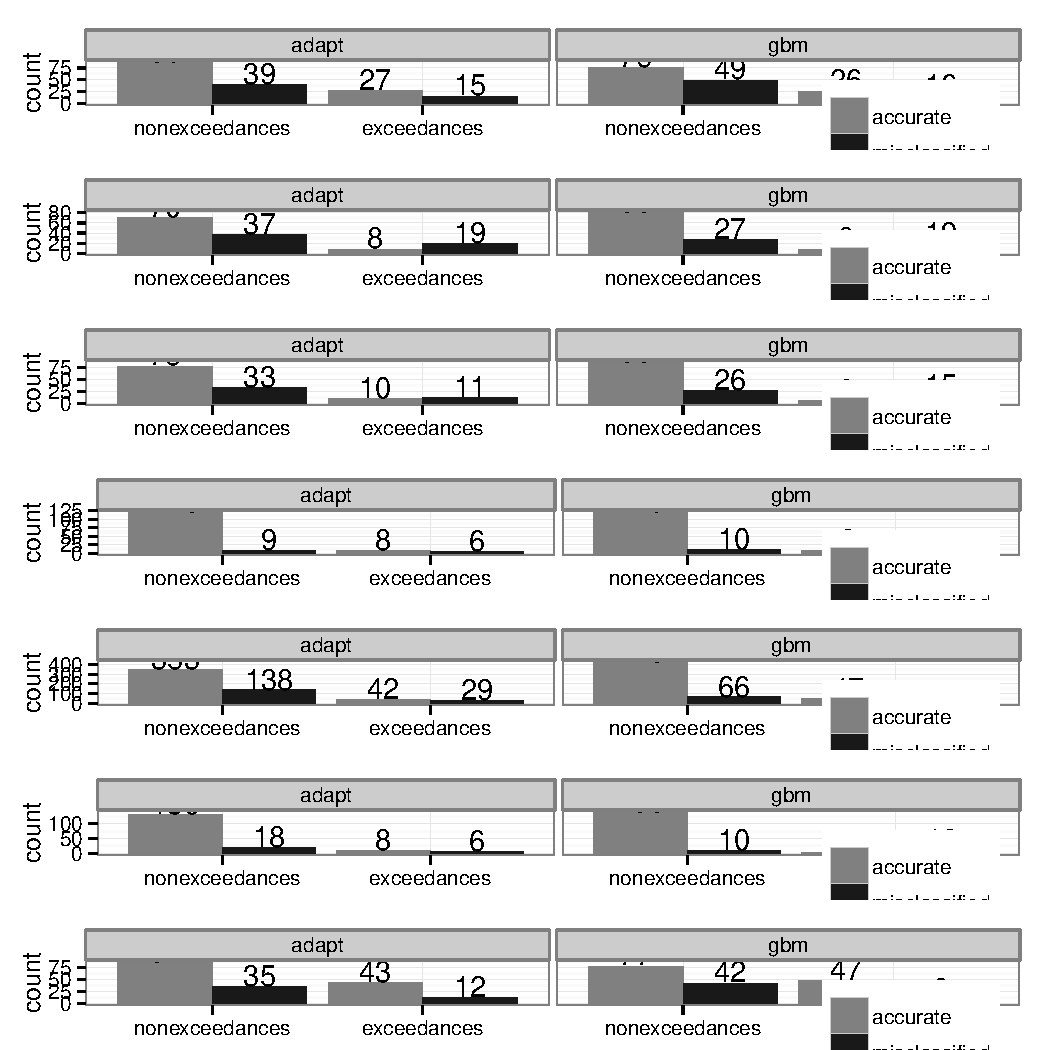
\includegraphics[width=\maxwidth]{figure/counts-barcharts} \caption[Mean ranks of the modeling techniques across the seven sites]{Mean ranks of the modeling techniques across the seven sites. At left are the mean ranks under leave-one-out cross validation, at the right are the mean ranks from leave-one-year-out cross validation.\label{fig:counts-barcharts}}
\end{figure}


\end{knitrout}


\subsection{Variable selection}

Several of the methods we tested do variable selection to pare the
number of covariates. We look here at how many variables were used
in the adaptive lasso models compared to the GBM models, which use
all the available covariates.

\begin{knitrout}
\definecolor{shadecolor}{rgb}{0.969, 0.969, 0.969}\color{fgcolor}\begin{kframe}


{\ttfamily\noindent\bfseries\color{errorcolor}{\#\# Error: error in evaluating the argument 'x' in selecting a method for function 'print': Error: object 'nvar.plot' not found}}\end{kframe}
\end{knitrout}


\section{Discussion}

In general, the GBM, and GBMCV, and AL techniques produced comparable
results that were superior to the other techniques in terms of predictive
performance. Since the GBMCV models take much longer to compute than
the others, we will not include them in our more detailed analysis
of the modeling results.

Which type of model is generally the best?

Under what conditions do some outperform others?

Relative value of overall best model versus methods that help trim
variables? e.g. how valuable is it to reduce number of predictors?
Further, which variables get cut? Expensive ones? Cheap ones?

How important is computational expense? Only an issue for model fitting
--- not prediction, but worth quantifying. E.g. if GBM with cross
validation takes hours, how much better? 

Model tuning for GBM versus GBM-CV --> notes on how GBM is faster
with similar performance (e.g. CV is overkill maybe)


\section{Acknowledgments}


\section{References}

\bibliographystyle{plainnat}
\addcontentsline{toc}{section}{\refname}\bibliography{0C__Users_wrbrooks_git_beauty_contest_references_beautycontest}

\end{document}
